\documentclass[11pt]{article}
%Importing custom commands
\usepackage{latex_goon/latex_goon}
\title{Transformers}
\author{Garrett Goon}
\begin{document}
%
%\maketitle

\vspace{1truecm}
%
%
\renewcommand{\thefootnote}{\fnsymbol{footnote}}
\begin{center}
{\huge \bf{Decoder-Only Transformers}}
\end{center}


\begin{abstract}

Notes on various aspects of Decoder-Only Transformers.

\end{abstract}

\tableofcontents


\renewcommand*{\thefootnote}{\arabic{footnote}}
\setcounter{footnote}{0}



\section{Decoder-Only Fundamentals \label{sec:decoder_only} }

The Transformers architecture \cite {vaswani2017attention}, which dominates Natural Language
Processing (NLP) as of July 2023, is a relatively simple architecture. There are various flavors and
variants of Tranformers, but we start by describing the decoder-only versions which underly the
GPT models \cite {gpt2radford2019language, gpt3brown2020language, gpt4openai2023}.


The full decoder-only architecture can be seen in Fig.~\ref{fig:transformers_architecture}. The
parameters which define the network can be found in App.~\ref{app:conventions}.
\begin{figure}[h]
    \centering
    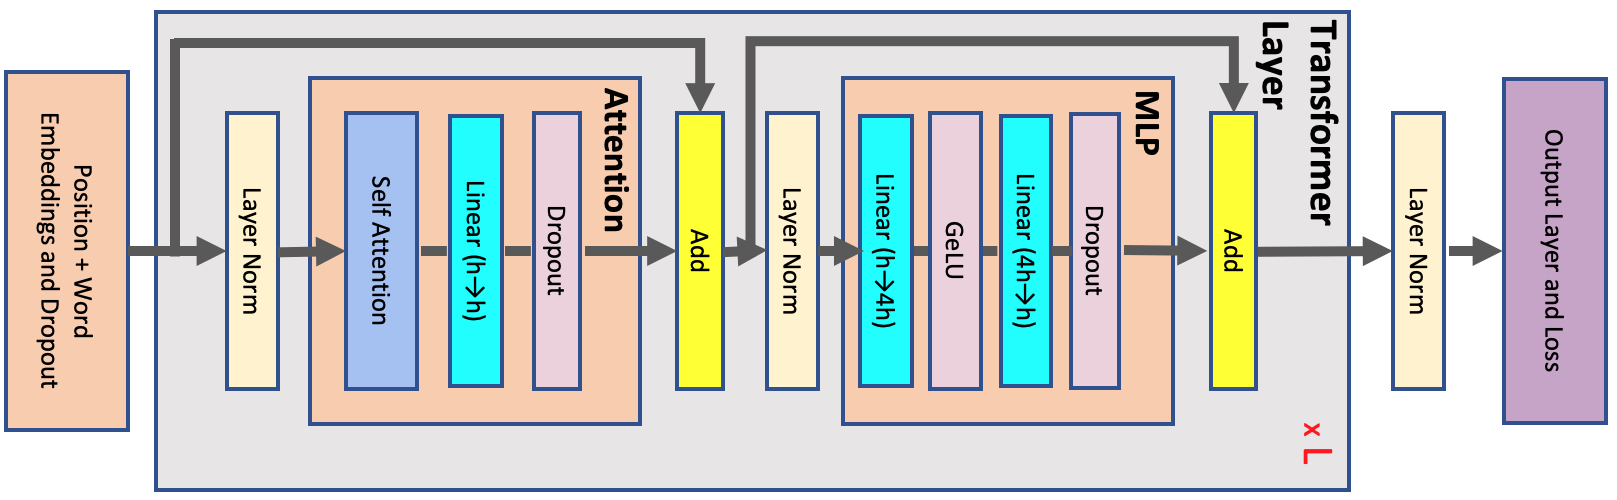
\includegraphics[scale=0.28]{figures/transformer-general.jpg}
    \caption{The full transformers architecture. Diagram taken from \cite{korthikanti2022reducing} }
    \label{fig:transformers_architecture}
\end{figure}


An outline of the mechanics:
\begin{enumerate}
    \item Raw text is \textbf{tokenized} and turned into a series of integers\footnote{There are
        about \href{https://github.com/ray-project/llm-numbers#131----average-tokens-per-word}{1.3 tokens per word}, on average.} whose values lie in \pyinline{range(V)}, with $ V $ the vocabulary
        size.
    \item The tokenized text is chunked and turned into \pyinline{(B, S)}-shaped (batch size and
        sequence length, respectively) integer tensors, $ x _{ bs } $.
    \item The \textbf{embedding layer} converts the integer tensors into continuous representations of shape
        \pyinline{(B, S, D)}, $ z _{ bsd } $, with $ D $ the size of the hidden dimension.
        \textbf{Positional encodings} have also been added to the tensor at this stage to help the
        architecture understand the relative ordering of the text.
    \item The $ z _{ bsd } $ tensors pass through a series of transformer blocks, each of which has
        two primary components:
        \begin{enumerate}
        \item In the \textbf{attention} sub-block, components of $ z _{ bsd } $ at different
            positions ($ s $-values) interact with each other, resulting in another \pyinline{(B, S, D)}-shaped
            tensor, $  z' _{ bsd } $.
        \item In the \textbf{MLP} block, each position in  $ z' _{ bsd } $ is processed
            independently and in parallel by a two-layer feed-forward network, resulting once more
            in a \pyinline{(B, S, D)}-shaped tensor.
        \end{enumerate}
        Importantly, there are \textbf{residual connections} around each of these\footnote{This
        gives rise to the concept of the \textbf{residual stream} which each transformer block reads
        from and writes back to repeatedly.} (the arrows in Fig.~\ref{fig:transformers_architecture}).
    \item Finally, we convert the \pyinline{(B, S, D)}-shaped
        tensors to \pyinline{(B, S, V)}-shaped ones, $ y _{ bsv } $. This is the role of
        the \textbf{language model head} (which is often just the embedding layer used in an inverse
        manner.)
    \item  The $ y _{ bsv } $ predict what the next token will be, having seen the \textbf{context}
        of the first $ s $ tokens in the sequence.
\end{enumerate}


Each batch (the $ b $-index) is processed independently. We omitted \pyinline{LayerNorm} and
\pyinline{Dropout} layers above, as well as the causal mask; these will be covered below as we step
through the architecture in more detail.


\subsection{Component Details \label{subsec:decoder_only_components} }

We break down the various components below.

\subsubsection{Embedding Layer and Positional Encodings \label{subsubsec:embedding_and_pe} }

The \textbf{embedding} layer is just a simple look up table: each of the \pyinline{range(V)} indices
in the vocabulary is mapped to a $ D $-dimensional vector via a large \pyinline{(V, D)}-shaped
table/matrix. This layer maps $ x _{ bs } \longrightarrow z _{ bsd } $. In \pyinline{torch}, this is
an \pyinline{nn.Embedding(V, D)} instance.

To each item in a batch, we add identical \textbf{positional encodings} to the vectors above with
the goal of adding fixed, position-dependent correlations in the sequence dimension which will
hopefully make it easier for the architecture to pick up on the relative positions of the inputs
\footnote{Positional encodings and the causal mask are the only components in the transformers
architecture which carry weights with a dimension of size $ S $; i.e. they are the only parts that
have explicit sequence-length dependence. A related though experiment: you can convince yourself
that if the inputs $ z_{ bsd } $
were just random noise, the transformers architecture would not be able to predict
the $ s $-index of each such input in the absence of positional encodings. } This layer maps $ z _{
bsd} \leftarrow z _{ bsd } + p _{ sd } $, with $ p _{ sd } $ the positional encoding tensor.

The above components require $ (V+S)D \approx VD $ parameters per layer.



\subsubsection{Layer Norm \label{subsubsec:layer_norm} }

The original transformers paper \cite{vaswani2017attention} put \pyinline{LayerNorm} instances after
the \textbf{attention} and \textbf{MLP} blocks, but now it is common \cite{xiong2020layer} to put
them before these blocks\footnote{Which makes intuitive sense for the purposes of stabilizing the
matrix multiplications in the blocks}.

The \pyinline{LayerNorm} operations acts over the sequence dimension. Spelling it out, given the
input tensor $ z _{ bsd } $ whose mean and variance over the $ s $-index are $ \mu _{ bd } $ and $
\sigma _{ bd } $, respectively, the \pyinline{LayerNorm} output is
\begin{align}
  z _{ bsd } &\leftarrow \left ( \frac{ z _{ bsd } - \mu _{ bd } }{ \sigma _{ bd } } \right )\times \gamma _{ d }
  + \beta _{ d } \equiv \LN _{ s } z _{ bsd}
\end{align}
where $ \gamma _{ d }, \beta  _{ d } $ are the trainable scale and bias parameters. In
\pyinline{torch}, this is a \pyinline{nn.LayerNorm(D)} instance.

Since there are two \pyinline{LayerNorm} instances in each transformer block, these components require
$ 2D $ parameters per layer.


\subsubsection{Attention \label{subsubsec:attn_layer} }

The \textbf{attention} layer is the most complex layer. It features $ A $  triplets\footnote{$ A $
must divide the hidden dimension $ D $ evenly.} of weight matrices\footnote{There are also bias
terms, but we will often neglect to write them explicitly or account for their (negligible)
parameter count.}  $ Q ^{ a } _{ d f }, K ^{ a } _{ df }, V ^{ a } _{ df }  $
where $ a \in \left \{ 0, \ldots, A-1 \right \} $ and $ f \in \left \{ 0, \ldots, D/A \right \} $.
From these, we form three different vectors:
\begin{align}
  q ^{ a }_{ bsf } &= z _{ bsd } Q ^{ a }_{ df } \ , \quad
  k ^{ a }_{ bsf } = z _{ bsd } K ^{ a }_{ df }  \ , \quad
  v ^{ a }_{ bsf } = z _{ bsd } V ^{ a }_{ df }
\end{align}
These are the \textbf{query, key, and value} tensors, respectively.

Using the above tensors, we will then build up an \textbf{attention map}  $ w ^{ a }_{ bss' } $
which corresponds to how much attention the token at position $ s $ pays to the token at
position $ s' $.  Because we have the goal of predicting the
next token in the sequence, we need these weights to be causal: the final prediction $ y _{ bsv } $
should only have access to information propagated from positions $ x _{ bs'v } $ with $ s' \le s $.
This corresponds to the condition that $ w ^{ a }_{ bss' } = 0  $ if  $ s' > s  $.

 These weights come from \pyinline{Softmax}-ed attention scores, which are just a normalized
 dot-product over the hidden dimension:
\begin{align}
    w ^{ a }_{ bss'd } &=\Sm _{ s' } \left (m _{ s s' }+\ q ^{ a }_{ bsf }k ^{ a }_{ bs'f } / \sqrt{D/A} \right
        )\ ,  \quad {\rm s.t.} \quad \sum_{s'}w ^{ a }_{ bdss' } =1
\end{align}
The tensor $ m _{  s s' } $ is the causal mask which zeroes out the relevant attention map
components above
\begin{align}
    m _{ s s' } &= \begin{cases}
            0 & s \le s' \nn
            -\infty &= s > s'
        \end{cases}
\end{align}
The $ \sqrt{D/A} $ normalization is motivated by demanding
that the variance of the \pyinline{Softmax} argument be 1 at initialization, assuming that other
components have been configured so that that the query and key components are i.i.d. from a Gaussian
normal distribution \footnote{However, in \cite{yang2022tensor} it is instead argued that no square
root should be taken in order to maximize the speed of learning via SGD.}.

The weights above are then passed through a dropout layer and used to re-weigh the \textbf{value} vectors and form the tensors
\begin{align}
  t ^{ a }_{ bsf }&=\Dr  \left (w ^{ a }_{ bdss' } \right ) v ^{ a }_{ bs'f }
\end{align}
and these $ A $ different \pyinline{(B, S, D/A)}-shaped tensors
are then concatenated along the $ f $-direction to re-form a \pyinline{(B, S, D)}-shaped
tensor\footnote{It is hard to come up with good index-notation for concatenation.}
\begin{align}
    u _{ bsd } &= {\rm Concat}^{ a }_{ fd } \left ( t ^{ a }_{ bsf }\right )\ .
\end{align}
Finally, another weight matrix $ O _{d' d } $ and dropout layer transform the output once again to get the final
output
\begin{align}
  z _{ bsd } &= \Dr \left (u  _{ bsd' } O _{ d'd }\right )\ .
\end{align}

For completeness, the entire operation in condensed notation with indices left implicit is:
\begin{align}
    z  &\leftarrow \Dr \left ({\rm Concat} \ \left ( \Dr \left (\Sm  \left ( \frac{ \left ( z \cdot Q ^{ a } \right )\cdot \left ( z \cdot K ^{ a } \right )}{ \sqrt{D/A} }
            \right)\right )\cdot z \cdot V ^{ a } \right ) \cdot O \right )
\end{align}
where all of the dot-products are over feature dimensions (those of size $ D $ or $ D/A $).
A nice\footnote{An example optimization: there is no need to form separate $ Q ^{ a },K ^{ a },V ^{
a} $ \pyinline{Linear} layers, one large layer which is later chunked is more efficient}, but
hopefully pedagogically useful, implementation of the attention layer is below:
\pyfile[firstline=10, lastline=57]{python/causal_attention.py}

The parameter count is dominated by the weight matrices which carry $ 4 D ^{ 2 } $ total parameters per layer.


\subsubsection{MLP \label{subsubsec:mlp} }

The feed-forward network is straightforward and corresponds to
\begin{align}
  z _{ bsd } &\leftarrow \phi \left ( z _{ bsd' }W ^{ 0 }_{ d'e } \right ) W ^{ 1 } _{ ed }
\end{align}
where $ W ^{ 0 } $ and $ W ^{ 1 } $ are \pyinline{(D, FD)}- and \pyinline{(FD, D)}-shaped matrices,
respectively (see App.~\ref{app:conventions} for notation) and $ \phi $ is a
non-linearity\footnote{The \pyinline{GeLU}
\href{https://pytorch.org/docs/stable/generated/torch.nn.GELU.html}{non-linearity} is common.}. The
implementation is straightforward: \pyfile[firstline=8, lastline=24]{python/mlp.py}

This bock requires $ 2 F D ^{ 2 } $ parameters per layer, only counting the contribution from
weights.


\subsubsection{Language Model Head \label{subsubsec:language_model_head} }


The layer which converts the \pyinline{(B, S, D)}-shaped outputs, $ z _{ bsd } $, to \pyinline{(B, S, V)}-shaped
predictions over the vocabulary, $  y _{ bsv } $, is the \textbf{Language Model Head}. It
is a linear layer, whose weights are usually tied to be exactly those of the initial embedding
layer of Sec.~\ref{subsubsec:embedding_and_pe}.


\subsubsection{All Together}
It is then relatively straightforward to tie everything together.  In code, we can first create a
transformer block like
\pyfile[firstline=10, lastline=30]{python/transformer_block.py}

And then the entire architecture: \pyfile[firstline=9, lastline=51]{python/decoder_only.py}

\subsection{Memory}


Understanding the memory cost of




\appendix


\section{Conventions and Notation}\label{app:conventions}


We loosely follow the conventions of \cite{korthikanti2022reducing} and denote the main Transformers
parameters by:
\begin{itemize}
\item $ B $: microbatch size
\item $ K $: the block size (maximum sequence length\footnote{In the absence of methods such as
    ALiBi \cite{ALiBi}  can be used to extend the sequence length at inference time.})
\item $ S $: input sequence length
\item $ V $: vocabulary size
\item $ D $: the hidden dimension size
\item $ L $: number of transformer layers
\item $ A $: number of attention heads
\item $ P $: pipeline parallel size
\item $ T $: tensor parallel size
\item $ F $: expansion factor for MLP layer (usually $ F=4 $)
\end{itemize}
Where it makes sense, we try to use the lower-case versions of these characters to denote the
corresponding indices on various tensors. For instance, an input tensor with the above batch size,
sequence length, and vocabulary size would be written as $ x _{ bsv } $, with $ b \in \left \{ 0,
\ldots, B - 1 \right \} $, $ s \in \left \{ 0, \ldots, S - 1\right \} $, and $  v \in \left \{ 0,
    \ldots, V -1\right \}$ in math notation, or as \mintinline{python}{x[b, s, v]} in code.  Typical
    transformers belong to the regime
\begin{gather}
V \gg D, S \gg L, A \gg P, T \ .  \label{app:eq:transformers_approxs}
\end{gather}


As indicated above,  we use zero-indexing. We also use \pyinline{python} code
throughout\footnote{Written in a style conducive to latex, e.g. no type-hints and pegagogy
prioritized.}  and
write all ML code using standard \pyinline{torch} syntax. To avoid needing to come up with new
symbols in math expressions we will often use expressions like $ x \leftarrow f(x) $ to refer to performing
a computation on some argument ($ x $) and assigning the result right back to the variable $ x $
again.

Physicists often joke (half-seriously) that Einstein's greatest contribution to physics was his
summation notation in which index-sums are implied by the presence of repeated indices and summation
symbols are entirely ommitted. For instance, the dot product between two vectors would be written as
\begin{align}
    \vec{x} \cdot \vec{y} &= \sum _{ i } x _{ i } y _{ i } \equiv x _{ i } y _{  i }
    \label{app:eq:einstein_sum}
\end{align}
We use similar notation which is further adapted to the common element-wise deep-learning
operations.  The general rule is that if a repeated index appears on one side of an equation, but
not the other, then a sum is implied, but if the same index appears on both sides, then it's an
element-wise operation. The Hadamard-product between two matrices $ A $ and $ B $ is just
\begin{align}
  C _{ ij } &= A _{ ij } B _{ ij }\ .
\end{align}

 We also put explicit indices on operators such as Softmax to help clarify the relevant
 dimension, e.g. we would write the softmax operation over the $ b $-ndex of some batched
 tensor $ x _{ bvd\ldots } $ as
 \begin{align}
     s _{ bvd\ldots } &= \frac{ e^{ x _{ bv d\ldots}  } }{ \sum _{ v = 0 } ^{  v= V-1 } e^{ x _{
     bvd\ldots } } } \equiv
     \Sm _{ v } \ x _{ bvd\ldots }
     \ , \label{app:eq:einstein_softmax}
 \end{align}
 indicating that the sum over the singled-out $ v $-index is gives unity.



 \section{TODO}


 \begin{itemize}
 \item Tokenizers
 \item Generation
 \item Activations
 \item Flash attention
 \item BERT family
 \item Residual stream
 \item Scaling laws
 \end{itemize}

\bibliographystyle{latex_goon/utphys}
\bibliography{bibliography}
\end{document}
